% Options for packages loaded elsewhere
\PassOptionsToPackage{unicode}{hyperref}
\PassOptionsToPackage{hyphens}{url}
%
\documentclass[
]{article}
\usepackage{amsmath,amssymb}
\usepackage{iftex}
\ifPDFTeX
  \usepackage[T1]{fontenc}
  \usepackage[utf8]{inputenc}
  \usepackage{textcomp} % provide euro and other symbols
\else % if luatex or xetex
  \usepackage{unicode-math} % this also loads fontspec
  \defaultfontfeatures{Scale=MatchLowercase}
  \defaultfontfeatures[\rmfamily]{Ligatures=TeX,Scale=1}
\fi
\usepackage{lmodern}
\ifPDFTeX\else
  % xetex/luatex font selection
\fi
% Use upquote if available, for straight quotes in verbatim environments
\IfFileExists{upquote.sty}{\usepackage{upquote}}{}
\IfFileExists{microtype.sty}{% use microtype if available
  \usepackage[]{microtype}
  \UseMicrotypeSet[protrusion]{basicmath} % disable protrusion for tt fonts
}{}
\makeatletter
\@ifundefined{KOMAClassName}{% if non-KOMA class
  \IfFileExists{parskip.sty}{%
    \usepackage{parskip}
  }{% else
    \setlength{\parindent}{0pt}
    \setlength{\parskip}{6pt plus 2pt minus 1pt}}
}{% if KOMA class
  \KOMAoptions{parskip=half}}
\makeatother
\usepackage{xcolor}
\usepackage{color}
\usepackage{fancyvrb}
\newcommand{\VerbBar}{|}
\newcommand{\VERB}{\Verb[commandchars=\\\{\}]}
\DefineVerbatimEnvironment{Highlighting}{Verbatim}{commandchars=\\\{\}}
% Add ',fontsize=\small' for more characters per line
\newenvironment{Shaded}{}{}
\newcommand{\AlertTok}[1]{\textcolor[rgb]{1.00,0.00,0.00}{\textbf{#1}}}
\newcommand{\AnnotationTok}[1]{\textcolor[rgb]{0.38,0.63,0.69}{\textbf{\textit{#1}}}}
\newcommand{\AttributeTok}[1]{\textcolor[rgb]{0.49,0.56,0.16}{#1}}
\newcommand{\BaseNTok}[1]{\textcolor[rgb]{0.25,0.63,0.44}{#1}}
\newcommand{\BuiltInTok}[1]{\textcolor[rgb]{0.00,0.50,0.00}{#1}}
\newcommand{\CharTok}[1]{\textcolor[rgb]{0.25,0.44,0.63}{#1}}
\newcommand{\CommentTok}[1]{\textcolor[rgb]{0.38,0.63,0.69}{\textit{#1}}}
\newcommand{\CommentVarTok}[1]{\textcolor[rgb]{0.38,0.63,0.69}{\textbf{\textit{#1}}}}
\newcommand{\ConstantTok}[1]{\textcolor[rgb]{0.53,0.00,0.00}{#1}}
\newcommand{\ControlFlowTok}[1]{\textcolor[rgb]{0.00,0.44,0.13}{\textbf{#1}}}
\newcommand{\DataTypeTok}[1]{\textcolor[rgb]{0.56,0.13,0.00}{#1}}
\newcommand{\DecValTok}[1]{\textcolor[rgb]{0.25,0.63,0.44}{#1}}
\newcommand{\DocumentationTok}[1]{\textcolor[rgb]{0.73,0.13,0.13}{\textit{#1}}}
\newcommand{\ErrorTok}[1]{\textcolor[rgb]{1.00,0.00,0.00}{\textbf{#1}}}
\newcommand{\ExtensionTok}[1]{#1}
\newcommand{\FloatTok}[1]{\textcolor[rgb]{0.25,0.63,0.44}{#1}}
\newcommand{\FunctionTok}[1]{\textcolor[rgb]{0.02,0.16,0.49}{#1}}
\newcommand{\ImportTok}[1]{\textcolor[rgb]{0.00,0.50,0.00}{\textbf{#1}}}
\newcommand{\InformationTok}[1]{\textcolor[rgb]{0.38,0.63,0.69}{\textbf{\textit{#1}}}}
\newcommand{\KeywordTok}[1]{\textcolor[rgb]{0.00,0.44,0.13}{\textbf{#1}}}
\newcommand{\NormalTok}[1]{#1}
\newcommand{\OperatorTok}[1]{\textcolor[rgb]{0.40,0.40,0.40}{#1}}
\newcommand{\OtherTok}[1]{\textcolor[rgb]{0.00,0.44,0.13}{#1}}
\newcommand{\PreprocessorTok}[1]{\textcolor[rgb]{0.74,0.48,0.00}{#1}}
\newcommand{\RegionMarkerTok}[1]{#1}
\newcommand{\SpecialCharTok}[1]{\textcolor[rgb]{0.25,0.44,0.63}{#1}}
\newcommand{\SpecialStringTok}[1]{\textcolor[rgb]{0.73,0.40,0.53}{#1}}
\newcommand{\StringTok}[1]{\textcolor[rgb]{0.25,0.44,0.63}{#1}}
\newcommand{\VariableTok}[1]{\textcolor[rgb]{0.10,0.09,0.49}{#1}}
\newcommand{\VerbatimStringTok}[1]{\textcolor[rgb]{0.25,0.44,0.63}{#1}}
\newcommand{\WarningTok}[1]{\textcolor[rgb]{0.38,0.63,0.69}{\textbf{\textit{#1}}}}
\usepackage{graphicx}
\makeatletter
\def\maxwidth{\ifdim\Gin@nat@width>\linewidth\linewidth\else\Gin@nat@width\fi}
\def\maxheight{\ifdim\Gin@nat@height>\textheight\textheight\else\Gin@nat@height\fi}
\makeatother
% Scale images if necessary, so that they will not overflow the page
% margins by default, and it is still possible to overwrite the defaults
% using explicit options in \includegraphics[width, height, ...]{}
\setkeys{Gin}{width=\maxwidth,height=\maxheight,keepaspectratio}
% Set default figure placement to htbp
\makeatletter
\def\fps@figure{htbp}
\makeatother
\setlength{\emergencystretch}{3em} % prevent overfull lines
\providecommand{\tightlist}{%
  \setlength{\itemsep}{0pt}\setlength{\parskip}{0pt}}
\setcounter{secnumdepth}{-\maxdimen} % remove section numbering
\ifLuaTeX
  \usepackage{selnolig}  % disable illegal ligatures
\fi
\IfFileExists{bookmark.sty}{\usepackage{bookmark}}{\usepackage{hyperref}}
\IfFileExists{xurl.sty}{\usepackage{xurl}}{} % add URL line breaks if available
\urlstyle{same}
\hypersetup{
  hidelinks,
  pdfcreator={LaTeX via pandoc}}

\author{}
\date{}

\begin{document}

\section{Homework 1}\label{homework-1}

\subsection{Dynamic Scope}\label{dynamic-scope}

Shell script is one of the few languages still in use which has dynamic
scoping. According to Wikipedia, \texttt{sh} was released in 1979 as a
replacement in Unix 7 for the Thompson shell\footnote{\url{https://en.wikipedia.org/wiki/Bourne_shell}
  Bourne shell}. Shell scripts are used to this day to automate common
sysadmin tasks and can be run on all major desktop platforms. In
addition to scripts, \texttt{sh} can also be used as a REPL and is a
common way to interface with UNIX-like systems.

\begin{Shaded}
\begin{Highlighting}[]
\CommentTok{\#!/bin/sh}
\VariableTok{x}\OperatorTok{=}\NormalTok{3}
\FunctionTok{func1 ()} \KeywordTok{\{} 
	\BuiltInTok{echo} \StringTok{"in func1: }\VariableTok{$x}\StringTok{"}
\KeywordTok{\}}
\FunctionTok{func2 ()} \KeywordTok{\{} 
	\BuiltInTok{local} \VariableTok{x}\OperatorTok{=}\NormalTok{9}
	\ExtensionTok{func1}
\KeywordTok{\}}

\ExtensionTok{func2}
\ExtensionTok{func1}
\end{Highlighting}
\end{Shaded}

The code above produces the following output:

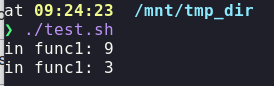
\includegraphics{/home/sebi/Documents/school/ZHAW/zhaw/Notizen/summaries/23HS/CSC 417 - Theory of Programming Languages/HW/res/Homework 1/image-20230831092447394.png}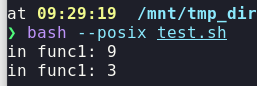
\includegraphics{/home/sebi/Documents/school/ZHAW/zhaw/Notizen/summaries/23HS/CSC 417 - Theory of Programming Languages/HW/res/Homework 1/image-20230831094300779.png}

As one can see, \texttt{func1} uses the definition of \texttt{x} of the
scope \texttt{func1} was invoked from. Since \texttt{func2} creates a
new \texttt{x}, this is the most recent definition of \texttt{x} and
\texttt{func1} proceeds to print \texttt{9}. After \texttt{func2} exits,
the definition of \texttt{x} of \texttt{func2} is popped from the stack
and the remaining and, now, most recent definition is \texttt{x=3}. This
is confirmed by the second output of \texttt{func1} which prints
\texttt{3}.

As a side node, while she-bang specifies \texttt{/bin/sh}, this is
usually symlinked to bash. Bash can also run in a -compliant mode with
the \texttt{-\/-posix} switch, which should be equivalent to the
standard set for \texttt{sh} scripts.

The example above is a slightly altered version taken from
\url{https://riptutorial.com/bash/example/8094/dynamic-scoping-in-action}.

\subsection{\texorpdfstring{Liskov Substitution Principle
}{Liskov Substitution Principle }}\label{liskov-substitution-principle}

A type defines properties and ways to access and modify those
properties. In OOP languages, this often comes in the form of methods
which access and modify fields.

A subtype has to be valid in the same context the super type is valid.
So, for example, passing a subtype to a function which expects the
subtype\textquotesingle s super type should still compile\footnote{\url{https://en.wikipedia.org/wiki/Subtyping}
  Subtyping}. This assumes that at least all public properties and the
public way to modify and access properties need to be present on a
subtype. However, a subtype might choose to change the implementation
detail of a method.

Inheritance is a way to "generate" subtypes by creating a type which
inherits all the properties and methods from its parents. Since all
properties are inherited, the subclass can be used in almost every
context the super class is valid. However, there are some exceptions to
this rule. For example, method parameters are contravariant, meaning
when overriding a method the parameter type may be substituted by its
super type, but not its subtype.\footnote{\url{https://en.wikipedia.org/wiki/Covariance_and_contravariance_(computer_science)\#Contravariant_method_parameter_type}
  Covariance and contravariance (computer science)}

The Liskov substitution principle states that the functionality of code
should be unchanged if an instance passed to that code is a subtype of
the required type.

A counter example of a structure which violates the Liskov substitution
principle is how Java implements read-only lists. In Java, a read-only
list can be created with the method
\texttt{\textless{}T\textgreater{}\ List\textless{}T\textgreater{}\ Collection.unmodifiableList(List\textless{}T\textgreater{}\ inputList)},
which will return a read-only list for the given \texttt{inputList}. The
returned list must be a subtype of
\texttt{List\textless{}T\textgreater{}} since
\texttt{Collection.unmodifiableList(...)} returns a
\texttt{List\textless{}T\textgreater{}} object.

\begin{Shaded}
\begin{Highlighting}[]
\CommentTok{/**}\NormalTok{ deletes all elements in the given list }\CommentTok{*/}
\DataTypeTok{void} \FunctionTok{deleteAll}\OperatorTok{(}\BuiltInTok{List}\OperatorTok{\textless{}}\BuiltInTok{String}\OperatorTok{\textgreater{}}\NormalTok{ list}\OperatorTok{)} \OperatorTok{\{}
\NormalTok{    list}\OperatorTok{.}\FunctionTok{clear}\OperatorTok{();}
\OperatorTok{\}}
\end{Highlighting}
\end{Shaded}

The code above defines a method which takes a list of strings and
deletes all elements in the list by calling the \texttt{List.clear()}
method. This code works great, assuming that the given list can be
modified. But if the argument is an unmodifiable list, then
\texttt{List.clear()} will throw an
\texttt{UnsupportedOperationException}\footnote{\url{https://docs.oracle.com/javase/8/docs/api/java/util/Collections.html\#unmodifiableList-java.util.List-}
  Collections.unmodifableList(...) JavaDoc}.

\begin{Shaded}
\begin{Highlighting}[]
\BuiltInTok{List}\OperatorTok{\textless{}}\BuiltInTok{String}\OperatorTok{\textgreater{}}\NormalTok{ readOnlyList }\OperatorTok{=} \BuiltInTok{Collections}\OperatorTok{.}\FunctionTok{unmodifiableList}\OperatorTok{(}\NormalTok{someList}\OperatorTok{);}
\FunctionTok{deleteAll}\OperatorTok{(}\NormalTok{readOnlyList}\OperatorTok{);} \CommentTok{// clear() will throw an UnsupportedOperationException}
\end{Highlighting}
\end{Shaded}

So when using the read-only subtype of
\texttt{List\textless{}T\textgreater{}}, the \texttt{deleteAll} method
breaks. In this case, this is because
\texttt{List\textless{}T\textgreater{}} defines methods which modify the
list (like \texttt{add(...)} or \texttt{clear()}). However, a read-only
implementation of \texttt{List\textless{}T\textgreater{}} cannot
possibly support these methods.

An example which shows how to implement a read-only list which follows
the Liskov substitution principle can be seen in C\#.

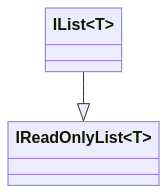
\includegraphics[width=1.73958in,height=\textheight]{16940112915012.png}

In the C\# world, an \texttt{IList}, the base interface for lists,
implements the \texttt{IReadOnlyList} interface. Meaning that
\texttt{IList} is a subtype of \texttt{IReadOnlyList}, where in the Java
world, a read-only list inherits from a \texttt{List}.

Because of this structure, the equivalent code in C\#
wouldn\textquotesingle t even compile.

\begin{Shaded}
\begin{Highlighting}[]
\DataTypeTok{void} \FunctionTok{DeleteAll}\OperatorTok{(}\NormalTok{List}\OperatorTok{\textless{}}\DataTypeTok{string}\OperatorTok{\textgreater{}}\NormalTok{ list}\OperatorTok{)} 
\OperatorTok{\{}
\NormalTok{    list}\OperatorTok{.}\FunctionTok{Clear}\OperatorTok{();}
\OperatorTok{\}}

\NormalTok{IReadOnlyList}\OperatorTok{\textless{}}\DataTypeTok{string}\OperatorTok{\textgreater{}}\NormalTok{ readOnlyList }\OperatorTok{=} \OperatorTok{...}
\FunctionTok{DeleteAll}\OperatorTok{(}\NormalTok{readOnlyList}\OperatorTok{);} \CommentTok{// this isn\textquotesingle{}t valid, since IReadOnlyList isn\textquotesingle{}t a subtype of List}
\end{Highlighting}
\end{Shaded}

\subsection{Stack and Heap}\label{stack-and-heap}

During the lifetime of a program, memory is allocated in multiple
location, including the stack and the heap.

A stack is a first-in-last-out collection, meaning that the first
element pushed on to the stack will be the last to be popped. Because of
this property, the stack is used for local variables and the return
address.

When a function is invoked, a new stack frame is pushed on the stack. A
frame contains space for local variables and the return address. When a
function returns, the top most stack frame will correspond to that
function. The CPU uses the return address to know where to jump back to.
Additionally, since the stack frame contains local variables, these
variables are automatically cleaned up when popping a stack
frame.\footnote{\url{https://en.wikipedia.org/wiki/Stack-based_memory_allocation}
  Stack-based memory allocation}

The frames with their return address and local data can be seen in the
following image.

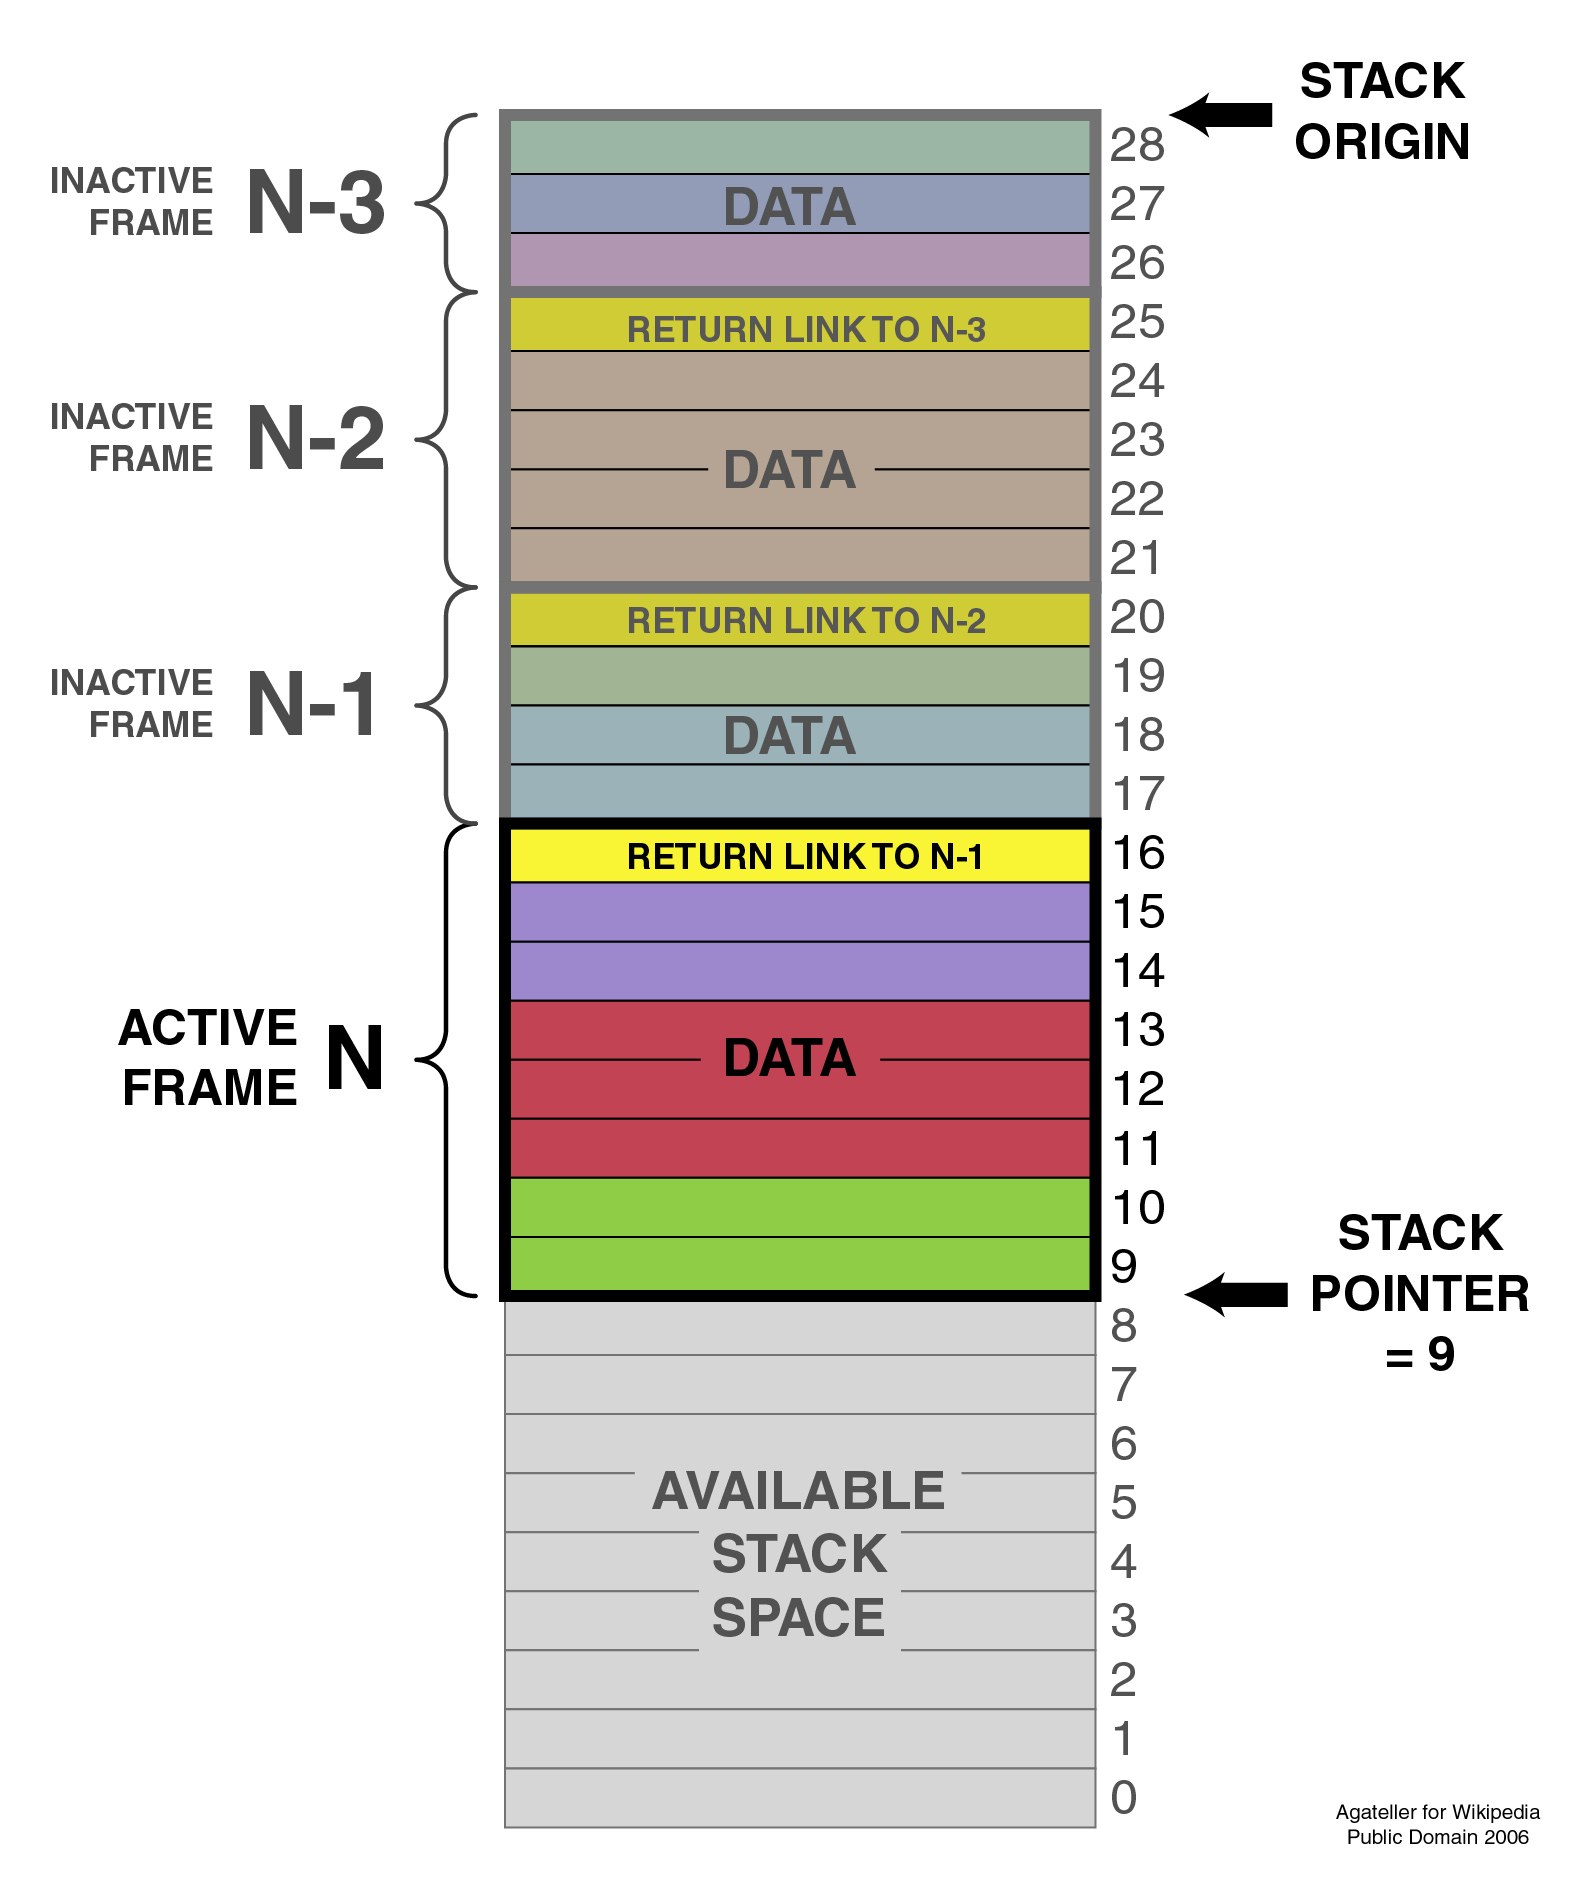
\includegraphics{/home/sebi/Documents/school/ZHAW/zhaw/Notizen/summaries/23HS/CSC 417 - Theory of Programming Languages/HW/res/Homework 1/ProgramCallStack2_en.png}

(Image is from
\url{https://commons.wikimedia.org/wiki/File:ProgramCallStack2_en.png})

The heap is a "place" in memory, where data which needs to be
independent of the current function being invoked. It is separate from
the stack and is not affected by function invocation and function
returning. Usually, long living objects and objects which are pointed to
by a pointer or reference are stored on the heap, as these object should
be deallocated when a function exists.

For example, an object managing a DB connection would (probably) be
stored on the heap, since it will live for most of the execution of the
program and will have multiple pointers pointing to it.

Which variables are stored on the heap and which are stored on the stack
is also dependent on the language implementation. For example, Java
always allocates objects on the heap, while a C or C++ programmer can
choose to allocate a struct on the stack.

If something is stored on the heap, there is typically a pointer on the
stack pointing to the location on the heap.

One important caveat with languages with manual memory management is,
that if a local variable is returned or otherwise accessible after a
function returned, it has to be allocated on the heap or moved to the
heap. Otherwise, it would be cleaned up after the function returns and
pointers to that object could point to random data.

\subsection{Reference Counting}\label{reference-counting}

Reference counting is a technique where each time a new reference is
made, a counter is incremented and each time a reference goes out of
scope (or is otherwise deallocated) the counter is decremented. When the
counter hits zero, the object is not reachable anymore and can be safely
deallocated. \footnote{\url{https://en.wikipedia.org/wiki/Reference_counting\#Garbage_collection}}

Reference counting is often used in languages without a garbage
collector in situations where an object is "owned" by multiple entities.

Rust implements reference counting in the
\texttt{Rc\textless{}T\textgreater{}} struct. Each time it is cloned,
the internal reference counter is incremented. When an
\texttt{Rc\textless{}T\textgreater{}} object is destroyed, then the
reference counter is decremented. \footnote{\url{https://doc.rust-lang.org/std/rc/index.html}}

\begin{Shaded}
\begin{Highlighting}[]
\KeywordTok{struct}\NormalTok{ Owner }\OperatorTok{\{}
\NormalTok{    name}\OperatorTok{:} \DataTypeTok{String}\OperatorTok{,}
\OperatorTok{\}}

\KeywordTok{struct}\NormalTok{ Gadget }\OperatorTok{\{}
\NormalTok{    id}\OperatorTok{:} \DataTypeTok{i32}\OperatorTok{,}
\NormalTok{    owner}\OperatorTok{:}\NormalTok{ Rc}\OperatorTok{\textless{}}\NormalTok{Owner}\OperatorTok{\textgreater{},}
\OperatorTok{\}}

\KeywordTok{fn}\NormalTok{ main() }\OperatorTok{\{}
    \KeywordTok{let}\NormalTok{ gadget\_owner}\OperatorTok{:}\NormalTok{ Rc}\OperatorTok{\textless{}}\NormalTok{Owner}\OperatorTok{\textgreater{}} \OperatorTok{=} \PreprocessorTok{Rc::}\NormalTok{new(}
\NormalTok{        Owner }\OperatorTok{\{}
\NormalTok{            name}\OperatorTok{:} \StringTok{"Gadget Man"}\OperatorTok{.}\NormalTok{to\_string()}\OperatorTok{,}
        \OperatorTok{\}}
\NormalTok{    )}\OperatorTok{;}

    \KeywordTok{let}\NormalTok{ gadget1 }\OperatorTok{=}\NormalTok{ Gadget }\OperatorTok{\{}
\NormalTok{        id}\OperatorTok{:} \DecValTok{1}\OperatorTok{,}
        \CommentTok{// increments the reference count in gadget\_owner}
\NormalTok{        owner}\OperatorTok{:} \PreprocessorTok{Rc::}\NormalTok{clone(}\OperatorTok{\&}\NormalTok{gadget\_owner)}\OperatorTok{,} 
    \OperatorTok{\};}

    \OperatorTok{\{}
        \KeywordTok{let}\NormalTok{ gadget2 }\OperatorTok{=}\NormalTok{ Gadget }\OperatorTok{\{}
\NormalTok{            id}\OperatorTok{:} \DecValTok{2}\OperatorTok{,}
            \CommentTok{// increments the reference count in gadget\_owner}
\NormalTok{            owner}\OperatorTok{:} \PreprocessorTok{Rc::}\NormalTok{clone(}\OperatorTok{\&}\NormalTok{gadget\_owner)}\OperatorTok{,}
        \OperatorTok{\};}
        \CommentTok{// gadet2 is dropped/deallocated since it goes }
        \CommentTok{// out of scope. This causes the reference count}
        \CommentTok{// in gadget\_owner to be decrement}
    \OperatorTok{\}}
    \CommentTok{// explicitly dropping gadget\_owner causing the reference}
    \CommentTok{// count to be decremented}
\NormalTok{    drop(gadget\_owner)}\OperatorTok{;} 

    \PreprocessorTok{println!}\NormalTok{(}\StringTok{"Gadget \{\} owned by \{\}"}\OperatorTok{,}\NormalTok{ gadget1}\OperatorTok{.}\NormalTok{id}\OperatorTok{,}\NormalTok{ gadget1}\OperatorTok{.}\NormalTok{owner}\OperatorTok{.}\NormalTok{name)}\OperatorTok{;}

    \CommentTok{// at the end of the function gadget1 is destroyed}
    \CommentTok{// which causes the reference count to go to zero}
    \CommentTok{// and the Owner instance will be destroyed}
\OperatorTok{\}}
\end{Highlighting}
\end{Shaded}

(example modified from
\url{https://doc.rust-lang.org/std/rc/index.html\#examples})

\subsection{Rust\textquotesingle s Memory
Management}\label{rusts-memory-management}

Rust uses the concept of ownership to decide when an object needs to be
deallocated.

The following ownership rules exist\footnote{\url{https://doc.rust-lang.org/stable/book/ch04-01-what-is-ownership.html}}
:

\begin{itemize}
\item
  Each value in Rust has an owner
\item
  There can only be one owner at a time
\item
  When the owner goes out of scope, the value will be
  dropped/deallocated
\end{itemize}

A simple \texttt{let\ x\ =\ y} transfers the ownership of \texttt{y} to
\texttt{x}. After that statement, \texttt{y} can no longer be used and
what was originally \texttt{y} will be deallocated once \texttt{x} goes
out of scope (assuming that the ownership isn\textquotesingle t
transferred further).

Since this would be extremely limiting, Rust allows mutable and
non-mutable references to objects. Rust calls this borrowing. When
borrowing a value, the ownership doesn\textquotesingle t change. One
important caveat, the object must remain in scope until there are no
references anymore.

\begin{Shaded}
\begin{Highlighting}[]
\KeywordTok{fn}\NormalTok{ main() }\OperatorTok{\{}
    \KeywordTok{let} \KeywordTok{mut}\NormalTok{ s }\OperatorTok{=} \DataTypeTok{String}\PreprocessorTok{::}\NormalTok{from(}\StringTok{"hello"}\NormalTok{)}\OperatorTok{;}
    \OperatorTok{\{}
        \CommentTok{// creates a non{-}mutable reference to s}
        \CommentTok{// while not transfering the ownership}
        \KeywordTok{let}\NormalTok{ s2 }\OperatorTok{=} \OperatorTok{\&}\NormalTok{s}\OperatorTok{;}
        \KeywordTok{let}\NormalTok{ s3 }\OperatorTok{=} \OperatorTok{\&}\NormalTok{s}\OperatorTok{;}
    \OperatorTok{\}}

    \OperatorTok{\{}
        \CommentTok{// creating a mutable reference}
        \KeywordTok{let}\NormalTok{ s4 }\OperatorTok{=} \OperatorTok{\&}\KeywordTok{mut}\NormalTok{ s}\OperatorTok{;}
    \OperatorTok{\}}
   
    \CommentTok{// transfer the ownership to s\_copy}
    \KeywordTok{let}\NormalTok{ mus s\_copy }\OperatorTok{=}\NormalTok{ s}\OperatorTok{;}
    
    \CommentTok{// the following wouldn\textquotesingle{}t compile since }
    \CommentTok{// s doesn\textquotesingle{}t have the ownership over the}
    \CommentTok{// String anymore.}
    \PreprocessorTok{println!}\NormalTok{(}\StringTok{"\{\}"}\OperatorTok{,}\NormalTok{ s)}\OperatorTok{;} 
\OperatorTok{\}}
\end{Highlighting}
\end{Shaded}

Because of this system, Rust can generate deallocation code for most
situations at compile time. For this reason, Rust has no garbage
collector, yet doesn\textquotesingle t require the programmer to
meticulously free every allocated object.

One downside of this system is that it explicitly disallows multiple
owners. However, there are situations where this is required. For these
cases, rust implements reference counting with
\texttt{Rc\textless{}T\textgreater{}} as an escape hatch. Importantly,
\texttt{Rc\textless{}T\textgreater{}} isn\textquotesingle t some kind of
primitive engraved in Rust\textquotesingle s type system. Rather, it is
built on top of the type system, and anybody can build a replacement if
they choose to do so.

As can be seen in the \texttt{Rc\textless{}T\textgreater{}} example in
the reference counting section, \texttt{Rc\textless{}T\textgreater{}}
wraps the value \texttt{T}. The three ownership rules are still upheld,
since each owner has their own \texttt{Rc\textless{}T\textgreater{}}
object which in the background uses \emph{unsafe} trickery to allow each
\texttt{Rc\textless{}T\textgreater{}} access to the underlying value.
\footnote{\url{https://doc.rust-lang.org/std/rc/index.html}}

\end{document}
